%=======================================================================
%
% ------------------------------------------------------------------------
% abnTeX2: Modelo de Trabalho Academico em conformidade com
% ABNT NBR 14724:2011: Informacao e documentacao - Trabalhos academicos
% ------------------------------------------------------------------------
% Customização IFC
% ------------------------------------------------------------------------
% Autor: Tiago Possato (tiago.possato@yahoo.com.br), baseado no modelo de Eliton Tiago
% Adaptação: Fábio Pinheiro (fabio.pinheiro@ifc.edu.br) e Henrique Pieri de Lima
% Versão: maio de 2026
% Codificação: UTF-8
% LaTeX: abnTeX2
%=======================================================================

\documentclass[
    12pt,
    oneside,
    a4paper,
    chapter=TITLE,
    section=TITLE,
    subsection=TITLE,
    english,
    brazil,
    sumario=tradicional,
]{abntex2-IFC}

% ---
% Pacotes fundamentais 
% ---
\usepackage{cmap}				% Mapear caracteres especiais no PDF
\usepackage{times}			    % Usa a fonte Times
\usepackage[T1]{fontenc}		% Selecao de codigos de fonte.fontenc
\usepackage[utf8]{inputenc}		% Codificacao do documento (conversão automática dos acentos)
\usepackage{lastpage}			% Usado pela Ficha catalográfica
\usepackage{indentfirst}		% Indenta o primeiro parágrafo de cada seção.
\usepackage{color}				% Controle das cores
\usepackage{graphicx}			% Inclusão de gráficos
\usepackage{amsfonts}			% Símbolos
%----Ajuste no alinhamento das listas
\usepackage{enumitem}
\setitemize[0]{itemindent=0.4cm,itemsep=0pt}
\setenumerate[0]{itemindent=0.5cm,itemsep=0pt}
%------
% ---
% Pacotes de citações
% ---
\usepackage[brazilian,hyperpageref]{backref}	 					  % Paginas com as citações na bibl

%% Comentários do professor
\usepackage[textwidth=18mm,colorinlistoftodos,prependcaption,textsize=tiny]{todonotes}
\setlength{\marginparwidth}{19mm}

\usepackage{xargs} 
\newcommandx{\incerto}[2][1=]{\todo[linecolor=red,backgroundcolor=red!25,bordercolor=red,#1]{#2}}
\newcommandx{\alterar}[2][1=]{\todo[linecolor=blue,backgroundcolor=blue!25,bordercolor=blue,#1]{#2}}
\newcommandx{\info}[2][1=]{\todo[linecolor=green,backgroundcolor=green!25,bordercolor=green,#1]{#2}}
\newcommandx{\melhorar}[2][1=]{\todo[linecolor=yellow,backgroundcolor=yellow!25,bordercolor=yellow,#1]{#2}}
\usepackage{soul,color}
%Lista de Acronimos
\usepackage[acronym, nomain, nonumberlist]{glossaries}
%\usepackage{glossaries-extra}
\makeglossaries

\usepackage[a4paper]{geometry}
%Referência
\usepackage[alf, 	
			 		abnt-emphasize=bf,
				    abnt-url-package=none,
				    abnt-repeated-title-omit=yes,
				    abnt-full-initials=yes,                                        %yes nome por extenso, no apenas iniciais
					abnt-etal-list=3												%abreviar com mais de 3 autores
]{abntex2/abntex2cite}				 														    % Citações padrão ABNT
\usepackage{lipsum}							   								       % para geração de dummy text
\usepackage{multirow}
\usepackage{float}
\usepackage{placeins}
\usepackage{setspace}
\usepackage{tabularx}

%\usepackage[none]{hyphenat}
%\captionsetup[table]{justification=raggedright}
% Configurações de aparência do PDF final
% alterando o aspecto da cor azul
\definecolor{blue}{RGB}{41,5,195}

% --- 
% Espaçamentos entre linhas e parágrafos 
% --- 
% O tamanho do parágrafo é dado por:
\setlength{\parindent}{2cm}
\linespread{1.5}

%Espaçamento depois dos títulos
\setlength{\afterchapskip}{\baselineskip}
% %\setlength{\afterchapskip}{\lineskip}

% Controle do espaçamento entre um parágrafo e outro:
\setlength{\parskip}{0cm}  % tente também \onelineskip

\hangcaption
\captionstyle[\raggedright]{}

%Estava mostrando nas referencias quais paginas estavam sendo referenciadas
\renewcommand{\backref}{}
\renewcommand*{\backrefalt}[4]{}

%Reduzir a fonte do caption
%\captionnamefont{\centering\ABNTEXfontereduzida}
%\captiontitlefont{\centering\ABNTEXfontereduzida}
%Ajuste nas listas de tabela, ilustrações e quadros
\setlength\cftbeforechapterskip{0pt}
% ---
% compila o indice
% ---
\makeindex
% ---

% Dados da capa e folha de rosto
% ---
% Informações de dados para CAPA e FOLHA DE ROSTO
% ---

\titulo{\uppercase{Análise do impacto de comportamentos de motoristas no tráfego urbano por meio de simulação computacional}}
\autor{\uppercase{Valdir Rugiski Junior}}
\local{Videira}
\data{2026}
\orientador[Orientador:]{Fábio José Rodrigues Pinheiro}
% \coorientador[Coorientador:]{Nome do coorientador}

\instituicao{Ministério da Educação\\
        Secretaria de Educação Profissional e Tecnológica\\
        Instituto Federal Catarinense\\
        Campus Videira}

\tipotrabalho{Trabalho de Conclusão de Curso}

% O preâmbulo deve conter o tipo do trabalho, o objetivo,
% o nome da instituição e a área de concentração.
\preambulo{Trabalho de Conclusão de Curso apresentado ao
Curso de graduação em Ciência da Computação do
Instituto Federal Catarinense – Campus Videira para
obtenção do título de bacharel em Ciência da Computação.

Orientador: \imprimirorientador

% Coorientador: \imprimircoorientador
}
% ---


\begin{document}

\frenchspacing

% ----------------------------------------------------------
% ELEMENTOS PRÉ-TEXTUAIS
% ----------------------------------------------------------

% CAPA
\imprimircapa

% FOLHA DE ROSTO
\imprimirfolhaderosto

% FOLHA DE APROVAÇÃO
% Mantida com dados provisórios até a definição da banca/data final.
\begin{folhadeaprovacao}

  \begin{center}
    \vspace*{-1.2cm}
    \textbf{\large\imprimirautor}

    \vspace*{\fill}\vspace*{\fill}\vspace*{\fill}

    \parbox{15cm}{
        \OnehalfSpacing
        \centering
        \large\textbf{\imprimirtitulo}
    }

    \vspace*{\fill}\vspace*{\fill}

    \hspace{.45\textwidth}
    \begin{minipage}{.5\textwidth}
        Este Trabalho de Curso foi julgado adequado para a obtenção
        do título de Bacharel em Ciência da Computação e aprovado em
        sua forma final pelo curso de graduação em Ciência da Computação
        do Instituto Federal Catarinense – Campus Videira.
    \end{minipage}

    \vspace*{\fill}
  \end{center}

  \vspace{-1cm}

  \begin{center}
    Videira (SC), dia de mês de 2026
  \end{center}

  \assinatura{
    \begin{center}
      \vspace{-0.7cm}
      \imprimirorientador \\
      Instituto Federal Catarinense – Campus Videira
    \end{center}
  }

  \begin{center}
    \textbf{BANCA EXAMINADORA}
  \end{center}

  \assinatura{
    \begin{center}
      \vspace{-0.7cm}
      NOME DO MEMBRO DA BANCA \\
      Instituto Federal Catarinense – Campus Videira
    \end{center}
  }

  \assinatura{
    \begin{center}
      \vspace{-0.7cm}
      NOME DO MEMBRO DA BANCA \\
      Instituto Federal Catarinense – Campus Videira
    \end{center}
  }

  \vspace*{1cm}

\end{folhadeaprovacao}


% FOLHA DE AUTORIZAÇÃO
% \begin{folhadeautorizacao}

  \begin{center}
  \vspace*{1 cm}
  \vspace{-2cm}
   \centering
\includegraphics[width=1.5cm]{brasaoRepublicaPeB.jpg}
   \vspace{-0.5 cm}
    {\large \SingleSpacing \imprimirinstituicao}
    \vspace{-0.5cm}
    \center{ \hrulefill}
    
     {\large \SingleSpacing \textbf{Autorização}}
    
    
    \vspace*{1 cm}
    
    \raggedleft{ Videira (SC), 19 de Novembro de 2016}
    \vspace*{0.5 cm}
    
   \end{center}
   


Eu, NOME SOBRENOME, regularmente matriculado na disciplina de Trabalho de Conclusão de Curso II - TC II do curso de Bacharel em Ciência da Computação, sob matrícula nº. XXXXXXX, pelo presente documento, autorizo o Instituto Federal Catarinense - IFC-Câmpus Videira, a utilizar o meu TC II intitulado "\imprimirtitulo", sob a orientação d Professor \imprimirorientador, para futuras informações e divulgações promovidas pelo Curso, e pelo Instituto, de forma institucional, em todo território nacional e internacional, sem fins comerciais, por qualquer meio de comunicação, tornando-o acessível a qualquer pessoa com interesse no trabalho.

A presente autorização substancia um consentimento de vontade e isenta de qualquer vício, feito de forma gratuita, e no gozo da minha capacidade civil, pelo que declaro nada me ser devido pelo curso de Ciência da Computação e pelo IFC-Câmpus Videira, ou seus representantes, em tempo algum, seja que título for, no que se refere, direta ou indiretamente, ao presente consentimento de uso da minha imagem e meu trabalho.

Declaro, ainda, que a utilização de meu nome e de meu trabalho, não constitui ofensa ou violação de meus direitos, nos termos do inciso X, do artigo 5o. da Constituição Federal.

Pelo presente também declaro ser de minha total responsabilidade o conteúdo de meu trabalho de conclusão de curso, descrito neste documento.

Os direitos e as obrigações aqui avençados transmitem-se aos meus herdeiros e sucessores.



  
   
   \vspace*{\fill}
   \vspace{-0.5 cm}
   
   \noindent Nome: \imprimirautor
   
   \vspace{0.25 cm}
   
   \noindent CPF: XXXXXXXXXXXXXX
   
   \vspace{0.25 cm}
   
   \noindent Assinatura: \hskip-3em\vtop{\vskip.05cm\hsize=5in \hrulefill}
   
   \vspace{0.5 cm}
   
    \begin{center}
    Rod. SC 135, KM 125 - Campo Experimental - CEP: 89560-000 - Videira - SC \\
    Fone: (49) 3533-4900 - http://www.ifc-videira.edu.br
    \end{center}

    \vspace*{1cm}
  
\end{folhadeautorizacao}

% Elementos opcionais. Habilitar quando forem preenchidos.
% \begin{dedicatoria}
 \vspace*{\fill}
 \noindent
  \raggedleft
 \begin{minipage}{.54\textwidth}
    Dedico este trabalho ...
   \end{minipage}
\end{dedicatoria}

% \begin{agradecimentos}

agradecimentos

\end{agradecimentos}

% RESUMO E ABSTRACT
% resumo em português
\begin{resumo}
\noindent
 
Neste trabalho
 \vspace{0.2cm}   
Palavras-chave: palavra 1. palavra 2. palavra 3
 
\end{resumo}
 
% resumo em inglês
\begin{resumo}[Abstract]	
\begin{otherlanguage*}{english}
\noindent 
 
This is the abstract of this work.
 
\vspace{0.2cm}
Key-words: Word 1. Word 2. Word 3
\end{otherlanguage*}
\end{resumo}


% LISTA DE ILUSTRAÇÕES
\pdfbookmark[0]{\listfigurename}{lof}
\listoffigures*
\cleardoublepage

% LISTA DE QUADROS
\pdfbookmark[0]{\listofquadrosname}{loq}
\listofquadros*
\cleardoublepage

% LISTA DE TABELAS
\pdfbookmark[0]{\listtablename}{lot}
% \listoftables*
% \cleardoublepage

% LISTA DE ABREVIATURAS E SIGLAS
\newacronym{ifc}{IFC}{Instituto Federal Catarinense}

\newacronym{ptc}{PTC}{Projeto de Trabalho de Conclusão de Curso}

\newacronym{tcc}{TCC}{Trabalho de Conclusão de Curso}

\newacronym[
    first={\textit{Simulation of Urban MObility} (SUMO)}
]{sumo}{SUMO}{\textit{Simulation of Urban MObility}}

\newacronym[
    first={\textit{eXtensible Markup Language} (XML)}
]{xml}{XML}{\textit{eXtensible Markup Language}}

\newacronym[
    first={\textit{Java Agent DEvelopment Framework} (JADE)}
]{jade}{JADE}{\textit{Java Agent DEvelopment Framework}}

\newacronym[
    first={\textit{Multi-Agent Transport Simulation} (MATSim)}
]{matsim}{MATSim}{\textit{Multi-Agent Transport Simulation}}

\newacronym[
    first={\textit{Verkehr In Städten -- SIMulationsmodell} (VISSIM)}
]{vissim}{VISSIM}{\textit{Verkehr In Städten -- SIMulationsmodell}}

\newacronym[
    first={\textit{Advanced Interactive Microscopic Simulator for Urban and Non-urban Networks} (Aimsun)}
]{aimsun}{Aimsun}{\textit{Advanced Interactive Microscopic Simulator for Urban and Non-urban Networks}}

\renewcommand*{\acronymname}{LISTA DE ACR\^ONIMOS}

\newglossarystyle{mylong}{%
    \setglossarystyle{long}%
    \renewenvironment{theglossary}%
        {\begin{longtable}[l]{@{}p{\dimexpr 2cm-\tabcolsep}p{0.8\hsize}}}
        {\end{longtable}}%
}

% Mantida a chamada utilizada no PTC, já validada no TeXPage.
\printglossary[toctitle=Acronymstype=acronym, style=mylong, title=LISTA DE ACR\^ONIMOS]

\cleardoublepage
\setcounter{figure}{0}
\setcounter{table}{0}

% SUMÁRIO
\pdfbookmark[0]{\contentsname}{toc}
\tableofcontents*
\cleardoublepage

% ----------------------------------------------------------
% ELEMENTOS TEXTUAIS
% ----------------------------------------------------------
\textual

% Capítulos já consolidados no PTC
\chapter{INTRODUÇÃO}

As orientações aqui apresentadas são baseadas em um conjunto de normas elaboradas pela ABNT. Além das normas técnicas a Biblioteca também elaborou  um guia para elaboração de trabalhos acadêmicos que está disponível na sua Homepage. < http://biblioteca.ifc.edu.br/normalizacao-de-trabalhos//>. 

Exemplos para referências: \cite{Alisson2025, Brasil2018, Das2023, Desdentado2025, Fernandes2025, Qureca2025, US2026}.

\section{Objetivos}

\subsection{Objetivo Geral}
	
Descrição...

\subsection{Objetivos Específicos} 

Descrição...

% 
%--------- FIM INTRODUÇÃO------------
%
\chapter{FUNDAMENTAÇÃO TEÓRICA}

\section{Tráfego urbano e mobilidade urbana}

A mobilidade urbana está ligada à forma como pessoas e veículos se deslocam dentro das cidades. Esse tema tem se tornado cada vez mais relevante, principalmente pelo crescimento das áreas urbanas e pelo aumento da quantidade de veículos em circulação. \citeonline{thakre_2024} destacam que o congestionamento urbano está associado a fatores como crescimento populacional, aumento da urbanização, limitações do transporte público, infraestrutura inadequada ou pouco planejada e aumento da quantidade de veículos particulares. Em muitos casos, esses fatores contribuem para problemas como lentidão, filas e aumento no tempo de deslocamento.

O congestionamento é um dos problemas mais visíveis nesse cenário. Ele pode ocorrer quando a quantidade de veículos em uma via se aproxima, ou até ultrapassa, sua capacidade de operação. No entanto, esse problema não depende apenas do número de veículos. Fatores como planejamento urbano, qualidade da infraestrutura, funcionamento do transporte coletivo, cruzamentos, semáforos e conversões também interferem diretamente no desempenho do tráfego \cite{thakre_2024}. Por isso, analisar o trânsito urbano exige observar não apenas a via em si, mas também a forma como ela é utilizada.

Outro ponto importante é que o tráfego urbano não se comporta de maneira totalmente previsível. Pequenas alterações, como uma redução de velocidade, uma conversão mal executada ou uma parada inesperada, podem causar impactos em outros veículos e gerar atrasos ao longo da via. Em regiões com maior fluxo, esses efeitos tendem a ser mais perceptíveis. A formação de filas, a redução da velocidade média e o aumento do tempo de viagem são exemplos de situações comuns quando há alguma limitação na capacidade da via ou interrupções frequentes no fluxo \cite{yu_2016}.

Entre as métricas utilizadas para avaliar o tráfego, o tempo de viagem é uma das mais importantes, pois está diretamente relacionado à experiência de deslocamento dos usuários. Esse tempo pode variar conforme o volume de veículos, as condições da via, a presença de semáforos, a ocorrência de pontos de retenção e também o comportamento dos motoristas \cite{yu_2016}. Assim, mesmo em um mesmo trecho urbano, diferentes condições de circulação podem produzir resultados bastante distintos.

O tráfego urbano também pode ser entendido como um sistema complexo, pois envolve diferentes elementos que interagem ao mesmo tempo. \citeonline{adewumi_2016}, ao discutirem a aplicação da teoria do caos na previsão de fluxos de tráfego em redes urbanas, destacam que esse tipo de sistema pode ser sensível às condições iniciais e às variações que ocorrem durante a circulação. Por isso, a análise da mobilidade urbana não deve considerar apenas a infraestrutura, mas também fatores como o volume de veículos, as regras de circulação, os cruzamentos, as conversões e as decisões tomadas pelos motoristas. A interação entre esses elementos ajuda a compreender como pequenas mudanças nas condições de tráfego podem produzir efeitos mais amplos no desempenho da via.

A modelagem e a simulação computacional são alternativas úteis para analisar sistemas de tráfego com diferentes condições de circulação, permitindo representar cenários e observar os efeitos de alterações sem interferir diretamente no ambiente real \cite{dorokhin_2020}. Essa abordagem também possibilita investigar como diferentes comportamentos de condução podem influenciar o desempenho do tráfego, aspecto relacionado diretamente à proposta deste trabalho \cite{zhai_2021}.

\section{Simulação computacional aplicada ao trânsito}

A simulação computacional é uma técnica utilizada para representar, de forma simplificada, o comportamento de um sistema real. No caso do trânsito, ela permite criar modelos que reproduzem determinadas condições de circulação, como volume de veículos, organização das vias, semáforos, cruzamentos e padrões de deslocamento. \citeonline{kotusevski_2009} destacam que a simulação computacional de tráfego é amplamente utilizada em pesquisas de modelagem, planejamento e desenvolvimento de redes de transporte. De forma semelhante, \citeonline{dorokhin_2020} apontam que a modelagem do movimento é um método utilizado em estudos de tráfego, planejamento e desenvolvimento de redes e sistemas de transporte.

Em estudos de tráfego urbano, a simulação permite testar diferentes cenários antes de qualquer intervenção prática. Por exemplo, é possível alterar o fluxo de veículos, modificar tempos semafóricos, bloquear uma via, mudar uma rota ou observar o comportamento do sistema em horários de maior demanda. Esse tipo de análise auxilia na compreensão dos efeitos que determinadas mudanças podem causar no desempenho da rede viária, sem que seja necessário realizar testes diretamente no ambiente urbano \cite{dorokhin_2020}.

Uma das principais vantagens da simulação é a possibilidade de avaliar cenários sob condições controladas. Em uma via real, o trânsito está sujeito a muitos fatores externos, como clima, acidentes, obras, eventos, comportamento imprevisível dos motoristas e variações na demanda ao longo do dia. \citeonline{kotusevski_2009} observam que experimentar diretamente em redes de tráfego reais nem sempre é prático, o que torna o ambiente simulado uma alternativa útil para investigar esse tipo de sistema. Assim, parte das variáveis pode ser controlada ou isolada, permitindo comparar os resultados de maneira mais organizada, principalmente quando se deseja avaliar o impacto de uma variável específica, como o comportamento dos motoristas.

O nível de detalhamento adotado em uma simulação depende do objetivo e da escala da análise. Diferentes abordagens podem ser utilizadas conforme o interesse esteja no comportamento geral do fluxo ou nas interações individuais entre os veículos \cite{algherbal_2025}. As principais formas de classificação desses modelos são apresentadas na seção seguinte.

Ao comparar diferentes ferramentas de simulação de tráfego, \citeonline{kotusevski_2009} mostram que esses sistemas podem variar em relação ao nível de detalhamento, à interface, à forma de construção da rede, à geração de rotas e aos tipos de saída produzidos. Essas diferenças reforçam a importância de escolher uma ferramenta compatível com os objetivos e as necessidades de cada estudo.

Além do planejamento urbano tradicional, a simulação de tráfego também vem sendo utilizada para avaliar soluções mais específicas, como intervenções sustentáveis e inovadoras em sistemas urbanos de entrega. \citeonline{su_2024} discutem o papel da simulação na análise de intervenções em entregas urbanas, mostrando que esse tipo de abordagem pode apoiar a avaliação de alternativas antes de sua aplicação em larga escala. Embora esse não seja o foco direto deste trabalho, o estudo reforça a utilidade da simulação como ferramenta de apoio à tomada de decisão em contextos urbanos.

No caso da análise do comportamento de motoristas, a simulação apresenta uma vantagem importante: ela permite comparar diferentes perfis de condução em um mesmo cenário. \citeonline{mecheva_2022} destacam que modelos de comportamento de motoristas são parte importante da simulação de tráfego e podem envolver parâmetros relacionados à forma de condução. Além disso, \citeonline{zhai_2021} indicam que características distintas dos condutores, como perfis tímidos e agressivos, podem afetar o desempenho do fluxo de tráfego. Assim, alterações em parâmetros relacionados à aceleração, frenagem, distância de seguimento, tempo de reação ou agressividade podem ser utilizadas para observar possíveis impactos no desempenho do tráfego em ambiente simulado.

\section{Modelos de simulação de tráfego}

Os modelos de simulação de tráfego são geralmente classificados, de acordo com o nível de detalhamento adotado, em macroscópicos, mesoscópicos e microscópicos \cite{dorokhin_2020}. Enquanto os modelos macroscópicos representam o fluxo de forma agregada, os microscópicos descrevem individualmente os veículos e suas interações, e os mesoscópicos ocupam uma posição intermediária entre essas abordagens. \citeonline{lopez_2018} também apresentam a categoria submicroscópica, na qual são representados elementos ainda mais detalhados do veículo. A escolha da abordagem depende do objetivo, da escala do cenário e do nível de detalhe necessário para a análise \cite{algherbal_2025}.

\subsection{Modelos macroscópicos}

Os modelos macroscópicos representam o tráfego de forma agregada, tratando o fluxo de veículos de maneira semelhante a um fluxo contínuo. \citeonline{lopez_2018} indicam que, nesse tipo de abordagem, são simuladas dinâmicas médias dos veículos, como a densidade do tráfego. Assim, o interesse principal está em variáveis como velocidade média, volume de tráfego e densidade de veículos. Em vez de acompanhar cada veículo separadamente, o modelo descreve o comportamento geral do fluxo em uma via ou em uma rede.

Esse tipo de modelo é útil quando o objetivo é analisar áreas maiores, como regiões urbanas extensas, rodovias ou redes viárias completas. Como trabalha com menor nível de detalhe, o modelo macroscópico tende a exigir menos esforço computacional e pode ser mais adequado para estudos em larga escala. Por outro lado, essa simplificação limita a análise de comportamentos individuais, como aceleração, frenagem, mudança de faixa e reação a outros veículos, aspectos mais associados à simulação microscópica \cite{lopez_2018}.

\citeonline{adacher_2018} discutem o uso do \textit{Cell Transmission Model} como uma abordagem macroscópica aplicada a redes urbanas. Nesse modelo, a via é dividida em segmentos e a evolução do fluxo é acompanhada ao longo do tempo, permitindo analisar fenômenos como a formação de congestionamentos e a propagação de filas.

\subsection{Modelos mesoscópicos}

Os modelos mesoscópicos ocupam uma posição intermediária entre os modelos macroscópicos e microscópicos. \citeonline{su_2024} indicam que esse tipo de simulação combina aspectos dos modelos macroscópicos e microscópicos, apresentando um nível de detalhe intermediário. De forma semelhante, \citeonline{dorokhin_2020} descrevem os modelos mesoscópicos como uma combinação entre a representação agregada dos fluxos e a consideração de elementos individuais do tráfego. Assim, o veículo pode existir como uma entidade separada no modelo, porém seu movimento e sua interação com os demais são descritos por relações mais simplificadas do que em uma simulação microscópica.

Essa abordagem pode ser interessante quando se deseja analisar redes maiores, mas ainda mantendo algum nível de representação dos deslocamentos individuais. Segundo \citeonline{dorokhin_2020}, os modelos mesoscópicos preservam um nível relativamente alto de detalhe na descrição da rede viária, mas simplificam a reprodução da dinâmica do fluxo, o que permite ampliar a escala da rede simulada mantendo maior velocidade de simulação. No entanto, por não representar todas as interações individuais com o mesmo detalhamento de um modelo microscópico, essa abordagem apresenta limitações para investigar decisões específicas de condução, como distância de seguimento, aceitação de lacunas ou mudança de faixa.

Apesar desse equilíbrio entre escala e detalhamento, a simplificação das interações individuais limita o uso de modelos mesoscópicos em análises que dependem de características específicas da condução. Nesses casos, abordagens com maior nível de detalhamento permitem representar de forma mais direta as interações entre veículos e motoristas \cite{dorokhin_2020}.

\subsection{Modelos microscópicos}

Os modelos microscópicos representam o tráfego em maior nível de detalhe. Nesse tipo de simulação, cada veículo é tratado individualmente, podendo possuir características próprias de movimento e interação. \citeonline{lopez_2018} indicam que, nos modelos microscópicos, cada veículo e sua dinâmica são modelados individualmente. Isso permite representar aspectos como aceleração, desaceleração, distância em relação ao veículo da frente, mudança de faixa, escolha de rota e resposta a elementos da via.

\citeonline{brambila_2008} destaca que, na simulação microscópica, o par veículo-motorista pode ser considerado uma entidade ativa do sistema. Essa característica é importante porque permite analisar como decisões individuais influenciam o comportamento coletivo do tráfego. Assim, o resultado da simulação não depende apenas de valores médios de fluxo, mas também das interações entre os veículos ao longo do tempo.

A movimentação e a interação dos veículos em modelos microscópicos são definidas por modelos comportamentais que representam diferentes situações da condução, como o acompanhamento do veículo à frente, a mudança de faixa e a entrada em fluxos de tráfego. Esses mecanismos permitem representar de forma mais detalhada as decisões tomadas durante o deslocamento e são discutidos na seção seguinte.

A principal vantagem da simulação microscópica, para este trabalho, está justamente na possibilidade de representar diferenças entre condutores. Como cada veículo pode receber parâmetros próprios, torna-se possível configurar perfis distintos de motoristas e observar como essas diferenças afetam o desempenho do tráfego. Por exemplo, motoristas com menor distância de seguimento, maior aceleração ou menor tempo de reação podem produzir resultados diferentes daqueles associados a perfis mais cautelosos.

Apesar das vantagens, a simulação microscópica também exige mais cuidado. Como o modelo trabalha com maior nível de detalhe, a construção do cenário, a definição da demanda de veículos e a escolha dos parâmetros de comportamento podem influenciar bastante os resultados. \citeonline{balakrishna_2007} destacam que modelos microscópicos dependem da definição de entradas e parâmetros, como fluxos de origem-destino e coeficientes associados a modelos de perseguição e mudança de faixa, para que os resultados representem adequadamente as condições analisadas. Além disso, \citeonline{cobos_2020} apontam que a calibração dos parâmetros continua sendo uma tarefa desafiadora em modelos microscópicos de fluxo de tráfego. Mesmo assim, para estudos que envolvem comportamento de motoristas, essa abordagem tende a ser mais adequada do que os modelos agregados.

Neste trabalho, a escolha pela simulação microscópica se justifica pelo objetivo de analisar o impacto de diferentes perfis de motoristas no desempenho do tráfego urbano. Como o foco está nas ações individuais dos condutores e nos efeitos dessas ações sobre o fluxo, é necessário utilizar um modelo capaz de representar veículos separadamente e permitir a alteração de parâmetros comportamentais. Dessa forma, a simulação microscópica oferece a base necessária para a construção dos cenários e para a comparação dos resultados obtidos.

\section{Simulação microscópica e comportamento de motoristas}

A possibilidade de representar individualmente os veículos torna a simulação microscópica adequada para estudos voltados ao comportamento dos motoristas. Nesse nível de modelagem, características relacionadas à condução podem ser incorporadas à dinâmica dos veículos, permitindo analisar como diferentes decisões e formas de reação influenciam suas interações ao longo da rede viária. \citeonline{brambila_2008} destaca que o par veículo-motorista pode ser considerado uma entidade ativa do sistema, sujeita às condições da via, aos veículos próximos e aos dispositivos de controle de tráfego.

\subsection{Modelos de comportamento na condução}

Entre os principais modelos utilizados em simulações microscópicas estão os modelos de perseguição de veículos, mudança de faixa e aceitação de lacunas. O modelo de perseguição de veículos, conhecido como \textit{car-following}, procura representar como um motorista ajusta sua velocidade de acordo com o veículo à frente. Essa decisão normalmente envolve fatores como distância entre veículos, velocidade relativa e capacidade de frenagem. \citeonline{gipps_1981} propôs um modelo comportamental de perseguição de veículos voltado à simulação computacional, considerando a segurança do condutor ao acelerar ou desacelerar durante o deslocamento.

Esse tipo de modelo é importante porque muitas situações de trânsito urbano envolvem reações sucessivas entre veículos. \citeonline{brambila_2008} explica que, nos modelos de perseguição, existe uma relação direta entre o veículo estudado e o veículo que ele segue, de modo que o motorista procura adaptar-se ao veículo da frente e evitar colisões. Assim, fatores como tempo de reação, distância mantida e diferença de velocidade influenciam a resposta do veículo perseguidor. Dependendo dessas condições, uma pequena alteração no movimento de um veículo pode afetar os veículos seguintes, contribuindo para redução de velocidade, lentidão ou formação de filas.

Além do movimento longitudinal, a mudança de faixa também é um comportamento relevante. \citeonline{brambila_2008} destaca que os modelos de mudança de pista procuram capturar as ações tomadas pelos motoristas durante esse tipo de manobra, considerando aspectos como segurança, trajetória e condições do tráfego. Em vias com mais de uma faixa, o motorista pode trocar de posição para ultrapassar, preparar uma conversão ou buscar uma faixa com melhor fluidez. Já a aceitação de lacunas, ou \textit{gap acceptance}, está relacionada à decisão de entrar em um fluxo, mudar de faixa ou realizar uma conversão quando existe um intervalo considerado seguro entre veículos \cite{brambila_2008}.

\subsection{Heterogeneidade entre motoristas}

Um ponto importante para este trabalho é que os motoristas não se comportam todos da mesma forma. Mesmo em uma mesma via e sob condições parecidas, diferentes condutores podem adotar velocidades, distâncias de seguimento e formas de reação bastante distintas. \citeonline{ossen_2011} analisam essa heterogeneidade no comportamento de \textit{car-following}, mostrando que diferenças entre motoristas podem ser observadas em dados reais de trajetórias veiculares.

A heterogeneidade entre motoristas também pode produzir efeitos no comportamento coletivo do tráfego. \citeonline{zhai_2021}, ao analisarem um modelo heterogêneo com motoristas de características distintas, mostram que diferentes composições de condutores podem alterar a estabilidade do fluxo. Esse resultado reforça a importância de considerar diferenças individuais em estudos que buscam analisar o desempenho do tráfego a partir do comportamento dos motoristas.

Além de influenciarem o comportamento do fluxo, essas diferenças individuais podem ser utilizadas para representar formas distintas de condução em ambientes simulados. \citeonline{witt_2019} abordam características comportamentais aplicáveis à simulação de tráfego, enquanto \citeonline{makridis_2023} discutem a caracterização da heterogeneidade dos motoristas a partir de diferenças observadas na dinâmica de condução. Essas abordagens mostram que a diversidade entre condutores pode ser traduzida em configurações computacionais, servindo como base para a definição de perfis de motoristas em ambientes simulados.

\subsection{Perfis de motoristas em ambientes simulados}

A definição de perfis de motoristas é uma forma prática de representar a diversidade comportamental dentro da simulação. Em vez de tentar reproduzir todos os detalhes psicológicos e sociais que influenciam um condutor real, o modelo utiliza parâmetros que afetam diretamente a condução. Entre esses parâmetros podem estar aceleração, desaceleração, velocidade desejada, tempo de reação, distância mínima de seguimento e tendência a aceitar ou rejeitar determinados espaços no tráfego.

\citeonline{andrade_2024} investigam a inferência de perfis de comportamento de motoristas em ambientes simulados com o uso de gêmeos digitais. Esse tipo de abordagem mostra que a simulação pode ser utilizada não apenas para reproduzir o trânsito, mas também para estudar e comparar padrões de condução. Embora a proposta deste trabalho seja mais simples, a ideia de analisar perfis comportamentais em ambiente controlado está diretamente relacionada.

No contexto deste trabalho, os perfis de motoristas são utilizados como uma abstração computacional. Isso significa que não se pretende afirmar que todos os condutores reais se encaixam perfeitamente em categorias fixas, como agressivo, normal ou cauteloso. A intenção é utilizar esses perfis como estratégia de experimentação, permitindo variar parâmetros de condução e observar seus efeitos sobre o tráfego. Essa simplificação é necessária para manter o estudo viável e, ao mesmo tempo, permitir uma análise comparativa.

A relação entre comportamento individual e desempenho coletivo é um dos pontos centrais da simulação microscópica. Estudos indicam que diferenças entre motoristas podem influenciar a dinâmica e a estabilidade do fluxo de tráfego \cite{zhai_2021,makridis_2023}. Dessa forma, a utilização de perfis de condução permite representar essas diferenças de maneira controlada e comparar seus efeitos sobre métricas como tempo médio de viagem, velocidade média, formação de filas e vazão. Essa abordagem serve de base para os experimentos realizados neste trabalho, nos quais diferentes composições de perfis foram avaliadas em um mesmo cenário simulado.

\section{Sistemas multiagentes aplicados à simulação de tráfego}

Os sistemas multiagentes são formados por entidades autônomas, chamadas agentes, que interagem entre si e com o ambiente em que estão inseridas. Em simulações de tráfego, essa perspectiva é útil porque permite compreender o trânsito como um sistema composto por múltiplos elementos que tomam decisões locais e influenciam o comportamento coletivo. \citeonline{doniec_2008} destacam que abordagens multiagentes podem ser utilizadas para representar fenômenos complexos, especialmente quando o comportamento global resulta das ações e interações entre agentes. No caso do tráfego urbano, essa ideia se relaciona à forma como motoristas, veículos, vias e regras de circulação interagem durante o deslocamento.

Na simulação de tráfego, os agentes podem representar diferentes elementos do sistema, como veículos, motoristas, semáforos ou sensores. Quando o foco está no comportamento dos condutores, o veículo ou o par veículo-motorista pode ser tratado como uma entidade que reage às condições ao redor, tomando decisões como acelerar, frear, manter distância, trocar de faixa ou escolher uma rota. \citeonline{gracian_2024} discutem modelos comportamentais de motoristas a partir de uma perspectiva baseada em agentes, destacando a importância desse tipo de abordagem para representar decisões de condução em ambientes de tráfego. Dessa forma, a modelagem baseada em agentes contribui para aproximar a simulação do caráter interativo e dinâmico do trânsito real.

Um aspecto importante dessa abordagem é que o comportamento global do tráfego resulta da interação entre múltiplos agentes, e não apenas de decisões isoladas. \citeonline{doniec_2008} apresentam um modelo comportamental multiagente voltado à simulação de tráfego viário, no qual as decisões individuais dos condutores e as interações entre veículos contribuem para a formação do comportamento coletivo do sistema.

A relação entre sistemas multiagentes e simuladores de tráfego também aparece em trabalhos que integram ferramentas específicas. \citeonline{soares_2014} apresentam uma plataforma que combina o simulador microscópico \gls{sumo} com o \textit{framework} multiagente \gls{jade}, com o objetivo de apoiar o desenvolvimento e a avaliação de soluções de tráfego baseadas em agentes. Embora este trabalho não tenha como objetivo implementar uma arquitetura multiagente completa, essa referência mostra que a aproximação entre simulação microscópica e conceitos de sistemas multiagentes já é explorada na literatura. Neste estudo, essa perspectiva é utilizada de forma conceitual, para fundamentar a representação de veículos e motoristas com características distintas dentro do ambiente simulado.

Assim, os conceitos de sistemas multiagentes contribuem para este trabalho ao oferecer uma perspectiva para compreender o tráfego como resultado das interações entre entidades com características distintas. Essa fundamentação complementa a abordagem microscópica adotada, permitindo relacionar as decisões individuais dos motoristas aos efeitos observados no comportamento coletivo do sistema, sem que seja necessária a implementação de uma arquitetura multiagente específica.

\section{Ferramentas de simulação de tráfego}

Existem diferentes ferramentas voltadas à simulação de tráfego, cada uma com características próprias. A escolha da ferramenta depende do tipo de estudo, do nível de detalhe necessário, da escala da rede, dos dados disponíveis e também de fatores práticos, como custo, documentação e facilidade de uso. Em trabalhos acadêmicos, esse último ponto acaba tendo bastante peso, pois nem sempre há acesso a softwares comerciais ou a bases de dados completas para calibração.

Entre as ferramentas utilizadas na área estão simuladores como \gls{vissim}, \gls{aimsun}, CORSIM, Paramics, TransModeler, \gls{matsim}, AnyLogic, Synchro/SimTraffic e \gls{sumo}. Algumas dessas ferramentas são comerciais e possuem interfaces gráficas mais completas, visualização em três dimensões e recursos avançados para aplicações profissionais. Outras são abertas ou voltadas a aplicações mais específicas, podendo exigir maior configuração manual, mas oferecendo maior flexibilidade para pesquisa e experimentação.

\citeonline{algherbal_2025} apresentam uma comparação entre diferentes softwares de simulação de tráfego, considerando critérios como tipo de modelo utilizado, disponibilidade, preço, sistema operacional, visualização e suporte a sistemas inteligentes de transporte. Os autores mostram que não existe uma única ferramenta superior para todos os casos. Cada simulador tende a ser mais adequado para determinados objetivos, como análise de interseções, rodovias, redes urbanas, transporte multimodal ou cenários envolvendo veículos conectados e autônomos.

Ferramentas como \gls{vissim} e \gls{aimsun} são bastante conhecidas em estudos de tráfego. O \gls{vissim} permite simulações microscópicas, mesoscópicas e macroscópicas, além de oferecer recursos visuais avançados e suporte a diferentes modos de transporte. O \gls{aimsun} também possui ampla aplicação em redes urbanas e rodoviárias, podendo trabalhar com diferentes níveis de modelagem. Apesar dessas vantagens, são ferramentas comerciais, o que pode limitar seu uso em trabalhos acadêmicos quando não há licença institucional disponível.

O CORSIM também é uma ferramenta tradicional de simulação microscópica, utilizada principalmente em estudos de corredores viários e redes urbanas. O Paramics, por sua vez, é conhecido pela representação tridimensional e pela capacidade de simular diferentes cenários de tráfego. Já o TransModeler oferece recursos para simulação em diferentes níveis de detalhe e pode ser utilizado em análises de planejamento e previsão. No entanto, assim como outras soluções comerciais, essas ferramentas podem apresentar barreiras relacionadas a custo, instalação, acesso e dependência de licença.

Outra ferramenta relevante é o \gls{matsim}, voltada à simulação multiagente de transporte. Ela é especialmente interessante para estudos em larga escala, envolvendo atividades diárias e deslocamentos em redes maiores. Porém, para o objetivo deste trabalho, que busca analisar o comportamento de motoristas em um cenário urbano simplificado, o foco está mais na simulação microscópica do movimento dos veículos do que na modelagem ampla de atividades urbanas.

Nesse contexto, o \gls{sumo} se apresenta como uma alternativa adequada. Segundo \citeonline{kotusevski_2009}, o \gls{sumo} é um simulador microscópico, \textit{open source} e portátil, projetado para lidar com redes rodoviárias. Além disso, permite a criação de redes de tráfego, a definição de rotas de veículos e a geração de arquivos de saída com informações úteis para análise. Esses aspectos tornam a ferramenta viável para pesquisas acadêmicas, principalmente quando se busca flexibilidade e baixo custo.

Uma característica importante do \gls{sumo} é a possibilidade de trabalhar com redes criadas manualmente, redes geradas automaticamente ou redes importadas de outras fontes. \citeonline{kotusevski_2009} destacam que o \gls{sumo} permite definir rotas por meio de diferentes estratégias, como fluxos, matrizes origem-destino e rotas descritas em arquivos \gls{xml}. Embora isso possa tornar a configuração inicial menos intuitiva do que em ferramentas comerciais com interface mais visual, também oferece maior controle sobre os cenários simulados.

Outro ponto relevante é que o \gls{sumo} produz diferentes tipos de saída, como informações sobre viagens, tempos de deslocamento, emissões, estados da rede, dados por faixa e dados por aresta \cite{kotusevski_2009}. Para este trabalho, essa possibilidade é importante porque permite obter métricas para comparar o desempenho do tráfego sob diferentes perfis de motoristas. Assim, dados como tempo de viagem, velocidade média, tempo parado e formação de filas podem ser utilizados na análise dos resultados.

\citeonline{lopez_2018} também apresentam o \gls{sumo} como uma ferramenta de simulação microscópica de tráfego amplamente utilizada em pesquisas. A ferramenta oferece recursos para simulação de redes urbanas, controle de veículos e integração com aplicações externas. Essa integração é relevante porque permite automatizar simulações, alterar parâmetros e coletar resultados por meio de scripts, o que se aproxima da proposta deste trabalho.

Com base nessas características, a escolha do \gls{sumo} considera tanto aspectos técnicos quanto práticos. Além de ser \textit{open source} e possuir documentação acessível, a ferramenta permite integração com Python, o que facilita a automação das simulações, a alteração de parâmetros e a organização dos resultados. Esses recursos são compatíveis com as necessidades dos experimentos realizados neste trabalho.

É importante reconhecer que o \gls{sumo} também possui limitações. Algumas configurações exigem edição de arquivos \gls{xml} e uso de linha de comando, o que pode tornar o processo menos simples no início, enquanto ferramentas comerciais podem oferecer interfaces mais amigáveis e recursos visuais mais elaborados. Mesmo assim, considerando o escopo deste trabalho, o acesso gratuito, a flexibilidade, a representação individual dos veículos, a possibilidade de configurar parâmetros relacionados à condução e a geração de dados para análise tornam o \gls{sumo} uma ferramenta adequada para o desenvolvimento das simulações propostas.

O Quadro~\ref{qua:ferramentas-simulacao} sintetiza as principais características das ferramentas discutidas nesta seção e destaca aspectos relevantes para a escolha do simulador utilizado no trabalho.

\begin{quadro}[H]
\centering
\caption{Comparação simplificada entre ferramentas de simulação de tráfego}
\label{qua:ferramentas-simulacao}
\small
\begin{tabular}{|p{2cm} | p{2.5cm} | p{3.8cm} | p{5.8cm}|}
\hline
\textbf{Ferramenta} & \textbf{Tipo de licença} & \textbf{Modelo predominante} & \textbf{Observação} \\
\hline
\gls{vissim} & Comercial & Microscópico & Possui interface avançada e recursos profissionais, mas depende de licença \\
\hline
\gls{aimsun} & Comercial & Micro, meso e macro & Adequado para diferentes escalas, porém com acesso limitado por custo \\
\hline
\gls{matsim} & \textit{Open source} & Multiagente & Forte em simulações de grande escala e atividades urbanas \\
\hline
\gls{sumo} & \textit{Open source} & Microscópico & Gratuito, flexível, integrável com Python e adequado à proposta deste trabalho \\
\hline
\end{tabular}

\par\vspace{0.25cm}
\begin{minipage}{\textwidth}
\footnotesize Fonte: Adaptado de \citeonline{kotusevski_2009}, \citeonline{lopez_2018} e \citeonline{algherbal_2025}.
\end{minipage}

\end{quadro}

\subsection{SUMO e modelos de comportamento veicular}

No \gls{sumo}, o comportamento dos veículos pode ser configurado por meio de modelos e parâmetros que influenciam sua movimentação e interação ao longo da rede. \citeonline{lopez_2018} destacam que a ferramenta permite representar individualmente a dinâmica dos veículos, característica que possibilita ajustar aspectos relacionados à condução e analisar seus efeitos durante a simulação.

Nos simuladores microscópicos, o movimento dos veículos depende de modelos comportamentais, como os modelos de perseguição de veículos, ou \textit{car-following}, responsáveis por representar como um veículo ajusta sua velocidade e sua distância em relação ao veículo à frente. \citeonline{mecheva_2022} discutem a modelagem do comportamento de motoristas com o uso do \gls{sumo} e Python, considerando diferentes modelos de \textit{car-following}, algoritmos de roteamento e parâmetros relacionados à condução. Entre os modelos disponíveis no simulador estão alternativas como Krauss e \textit{Intelligent Driver Model} (IDM). Embora este trabalho não tenha como objetivo comparar diferentes modelos internos do simulador, a escolha do modelo de comportamento veicular e de seus parâmetros faz parte da configuração da simulação e pode influenciar os resultados obtidos.

Neste trabalho, o \gls{sumo} será utilizado como ferramenta para construir um cenário urbano simplificado e configurar perfis distintos de motoristas. A escolha dos parâmetros associados a esses perfis considerou as possibilidades do simulador, a literatura sobre comportamento de motoristas, os parâmetros configuráveis da ferramenta e testes preliminares no cenário construído. Assim, a discussão sobre modelos de comportamento veicular no \gls{sumo} contribui para delimitar a base técnica da simulação, sem ampliar o escopo para uma comparação aprofundada entre modelos de \textit{car-following}.

\subsection{Parametrização do comportamento de motoristas no SUMO}

A representação de diferentes perfis de motoristas em uma microssimulação depende da combinação de parâmetros que controlam aspectos distintos da condução. Esses parâmetros não devem ser interpretados isoladamente como características completas de um condutor. \citeonline{makridis_2023}, por exemplo, destacam que a aceleração, sozinha, não é suficiente para caracterizar de forma adequada a agressividade de um motorista, pois o valor observado também depende das características do veículo e da condição de velocidade. Dessa forma, a construção de perfis em ambiente simulado é mais adequada quando considera um conjunto coerente de parâmetros.

No \gls{sumo}, o movimento longitudinal dos veículos pode ser representado por diferentes modelos de \textit{car-following}. O modelo Krauss é utilizado como modelo padrão do simulador e trabalha com parâmetros relacionados à distância e ao tempo de seguimento, além das capacidades de aceleração e desaceleração. Entre os parâmetros configuráveis estão \textit{tau}, associado ao intervalo temporal desejado em relação ao veículo à frente, \textit{minGap}, relacionado à distância mínima mantida em situação de parada, e os parâmetros \textit{accel} e \textit{decel}, que representam capacidades de aceleração e desaceleração do veículo. Estudos que utilizam o SUMO mostram que esses valores podem ser ajustados conforme o comportamento que se pretende representar \cite{mecheva_2022,schrader_2024a}.

A utilização conjunta desses parâmetros aparece em trabalhos voltados à diferenciação de estilos de condução. \citeonline{camlica_2022} configuraram comportamentos normal e agressivo no SUMO alterando, entre outros elementos, aceleração, desaceleração, distância mínima, \textit{tau}, impaciência e assertividade na mudança de faixa. Em outro estudo, \citeonline{yavuz_2025} utilizaram comportamentos defensivo, normal e agressivo e associaram os perfis mais defensivos a maiores valores de \textit{headway} e distância mínima, enquanto perfis mais agressivos foram representados com menores espaçamentos e maior capacidade de aceleração. Embora os cenários e os valores adotados nesses estudos sejam específicos de seus experimentos, a direção dessas variações fornece uma referência para a construção de perfis sintéticos em simulação.

O comportamento lateral também pode ser diferenciado. No modelo de mudança de faixa LC2013, o parâmetro \textit{lcAssertive} está relacionado à disposição do veículo em aceitar espaços menores à frente e atrás na faixa de destino. Valores mais elevados tornam a mudança de faixa mais assertiva, enquanto valores menores representam uma postura mais conservadora \cite{yavuz_2025}. Esse tipo de configuração permite complementar os parâmetros longitudinais e representar diferenças que não se limitam à aceleração ou à distância de seguimento.

Nas interseções, a decisão de avançar diante de fluxos conflitantes envolve ainda mecanismos específicos de prioridade e aceitação de lacunas. \citeonline{erdmann_2014} descrevem o modelo de interseções do SUMO e apresentam o conceito de impaciência como um fator que altera a disposição do veículo em realizar a manobra mesmo quando isso exige maior desaceleração dos veículos prioritários. O modelo também considera o aumento da impaciência conforme o tempo de espera. De forma aplicada, \citeonline{bagheri_2023} discutem a influência de parâmetros de aceitação de lacunas, aceleração, desaceleração e impaciência sobre o comportamento de veículos em interseções não semaforizadas.

Esses estudos mostram que a definição de perfis de condução no SUMO não depende de um único indicador. A combinação de parâmetros de seguimento, aceleração, velocidade desejada, mudança de faixa e interação em interseções permite construir comportamentos distintos de forma controlada. Neste trabalho, essa parametrização é utilizada como uma abstração computacional para representar os perfis cauteloso, normal e agressivo. Os valores efetivamente adotados e os critérios utilizados para diferenciá-los são apresentados posteriormente, no capítulo dedicado à configuração dos experimentos.

\section{Trabalhos correlatos}

Esta seção apresenta alguns trabalhos relacionados à simulação de tráfego, modelagem de comportamento de motoristas e análise de perfis de condução. A intenção não é fazer uma revisão exaustiva sobre todos os estudos existentes na área, mas destacar pesquisas que se aproximam da proposta deste trabalho em algum aspecto, seja pelo uso de simulação microscópica, pela análise de comportamento de condutores ou pela representação de perfis distintos de motoristas.

\citeonline{zhai_2021} propuseram um modelo heterogêneo de fluxo de tráfego considerando características de motoristas tímidos e agressivos. O trabalho parte da ideia de que muitos modelos tratam os condutores como homogêneos, apesar de, em situações reais, os motoristas apresentarem diferenças de comportamento. Para representar essa variação, os autores utilizam uma taxa de penetração de motoristas com diferentes características e analisam seus efeitos sobre a estabilidade do fluxo de veículos. Esse estudo se aproxima da proposta deste trabalho por considerar que perfis distintos de condução podem alterar o desempenho do tráfego. A diferença é que, enquanto o estudo de Zhai, Wu e Luo trabalha com um modelo matemático de fluxo heterogêneo, este trabalho analisa os efeitos desses perfis em um cenário urbano simulado com apoio de uma ferramenta de microssimulação.

\citeonline{mecheva_2022} investigaram a modelagem do comportamento de motoristas em simulação de tráfego utilizando \gls{sumo} e Python. O trabalho propõe uma metodologia para definir parâmetros de modelos de comportamento com base em dados de tráfego, considerando modelos de perseguição de veículos e algoritmos de roteamento. Essa pesquisa é relevante porque mostra a possibilidade de utilizar o \gls{sumo} em conjunto com scripts externos para configurar, executar e analisar simulações relacionadas ao comportamento de condução. Em relação ao presente trabalho, há proximidade no uso do \gls{sumo} e na preocupação com parâmetros comportamentais. No entanto, a proposta aqui é mais direcionada à comparação entre perfis de motoristas em um recorte urbano simplificado.

\citeonline{andrade_2024} exploraram a inferência de perfis de comportamento de motoristas em ambientes simulados, utilizando gêmeos digitais e dados de telemetria. O estudo considera condições de condução cautelosa e agressiva, buscando identificar padrões de comportamento a partir dos dados coletados durante a simulação. Esse trabalho se relaciona diretamente com a proposta deste trabalho, pois também trata da diferenciação entre perfis de motoristas em ambiente controlado. A principal diferença está no objetivo: enquanto Andrade et al. buscam inferir perfis a partir de dados de simulação, este trabalho define os perfis previamente para observar como eles influenciam o desempenho do tráfego urbano.

\citeonline{chah_2024} desenvolveram uma base de comportamentos simulados de motoristas utilizando o simulador \gls{sumo}. O trabalho considera a geração de dados associados a estilos de condução, como comportamentos normais ou perigosos, com o objetivo de apoiar aplicações relacionadas à segurança viária e serviços baseados no comportamento do condutor. A relação com este trabalho está no uso do \gls{sumo} para representar comportamentos distintos de motoristas. No entanto, enquanto Chah et al. concentram-se na construção de uma base de dados de comportamentos simulados, este estudo busca avaliar os efeitos desses comportamentos sobre métricas de desempenho do tráfego, como tempo de viagem, velocidade média, filas e vazão.

\citeonline{park_2019} analisaram os impactos da direção agressiva sobre segurança e mobilidade em rodovias, utilizando uma abordagem de simulação multiagente associada a modelo microscópico de tráfego. O estudo busca compreender como eventos de condução agressiva podem afetar o fluxo e aumentar riscos em ambientes viários. Embora o cenário analisado seja diferente do proposto neste trabalho, pois está voltado a rodovias, a pesquisa é relevante por relacionar comportamento agressivo, simulação e desempenho do tráfego. A principal diferença é que este trabalho foi aplicado a um cenário urbano simplificado, com foco na comparação entre perfis de condução e seus efeitos sobre a fluidez do trânsito.

De forma geral, os trabalhos analisados mostram que a modelagem do comportamento de motoristas é um tema relevante em simulações de tráfego. Alguns estudos focam em modelos matemáticos de fluxo heterogêneo, outros na identificação de perfis de condução, na geração de bases simuladas ou na análise de comportamentos agressivos em cenários específicos. Em comum, esses trabalhos reforçam que considerar diferenças entre condutores pode tornar a análise de tráfego mais realista do que assumir um comportamento único para todos os veículos.

A proposta deste trabalho se diferencia por buscar uma análise aplicada em um cenário urbano simplificado, baseado no entorno da Praça Nereu Ramos, em Videira/SC, utilizando simulação microscópica para comparar o impacto de diferentes perfis de motoristas sobre métricas de desempenho do tráfego. Assim, o foco não está apenas em representar comportamentos individuais, mas em observar como diferentes composições desses perfis podem influenciar o funcionamento geral do sistema simulado.

O Quadro~\ref{qua:trabalhos-correlatos} apresenta uma síntese dos principais trabalhos correlatos discutidos nesta seção, destacando seu foco, sua relação com esta pesquisa e suas principais diferenças.

\begin{quadro}[htbp]
\centering
\caption{Síntese dos trabalhos correlatos}
\label{qua:trabalhos-correlatos}
\small
\begin{tabular}{|p{3.5cm} | p{3.5cm} | p{3.5cm} | p{4cm}|}
\hline
\textbf{Trabalho} & \textbf{Foco principal} & \textbf{Relação com este\newline trabalho} & \textbf{Diferença principal} \\
\hline
\citeonline{zhai_2021} & Motoristas tímidos e agressivos em fluxo heterogêneo & Considera perfis distintos de condutores & Abordagem mais matemática, sem foco em cenário urbano real \\
\hline
\citeonline{mecheva_2022} & Modelagem de comportamento no \gls{sumo} & Usa \gls{sumo} e parâmetros comportamentais & Foco em metodologia de parametrização \\
\hline
\citeonline{andrade_2024} & Inferência de perfis em ambiente simulado & Trabalha com perfis cauteloso e agressivo & Busca inferir perfis, enquanto este trabalho define perfis previamente \\
\hline
\citeonline{chah_2024} & Base de comportamentos simulados no \gls{sumo} & Usa \gls{sumo} para gerar comportamentos distintos & Foco em base de dados, não em desempenho do tráfego urbano \\
\hline
\citeonline{park_2019} & Direção agressiva, segurança e mobilidade & Relaciona comportamento agressivo e simulação & Cenário rodoviário, não urbano \\
\hline
\end{tabular}

\par\vspace{0.25cm}
\begin{minipage}{\textwidth}
\footnotesize Fonte: Elaborado pelo autor.
\end{minipage}

\end{quadro}

% 
%--------- FIM DESENVOLVIMENTO------------
%

% ----------------------------------------------------------
% DESENVOLVIMENTO DO TC
% ----------------------------------------------------------
% Os arquivos abaixo foram preservados do PTC como referência textual,
% mas não são incluídos nesta versão do TC porque serão reestruturados
% para descrever o trabalho efetivamente realizado.
%
% \chapter{METODOLOGIA CIENTÍFICA}

\section{Classificação da pesquisa}

Este trabalho caracteriza-se como uma pesquisa aplicada, de abordagem quantitativa e com caráter experimental. Segundo \citeonline{gil_2002}, pesquisas podem estar associadas a razões de ordem prática, relacionadas à produção de conhecimento com vistas à sua aplicação. Nesse sentido, este trabalho possui natureza aplicada por utilizar conceitos e ferramentas de simulação computacional para investigar um problema relacionado ao tráfego urbano. O objetivo não é desenvolver uma nova ferramenta de simulação, mas utilizar uma ferramenta existente como apoio para analisar como diferentes comportamentos de motoristas podem influenciar o desempenho do tráfego em um cenário urbano simulado.

A abordagem quantitativa se justifica pelo uso de métricas numéricas para comparar os resultados obtidos nas simulações. Entre essas métricas, poderão ser considerados o tempo médio de viagem, a velocidade média, o tempo parado, a formação de filas e a vazão de veículos. Esses dados permitirão comparar os cenários simulados de forma objetiva, observando diferenças entre configurações de fluxo e perfis de motoristas.

A pesquisa também possui caráter experimental, pois serão criados cenários controlados de simulação nos quais determinadas variáveis serão alteradas. Segundo \citeonline{gil_2002}, a pesquisa experimental envolve a seleção de variáveis capazes de influenciar o objeto de estudo e a definição de formas de controle e observação de seus efeitos. Neste trabalho, as principais variáveis estarão relacionadas ao fluxo de veículos e aos parâmetros de comportamento dos motoristas. Ao manter uma mesma rede viária e modificar esses fatores, será possível observar como cada configuração interfere no desempenho geral do tráfego.

É importante destacar que o trabalho não pretende reproduzir com precisão absoluta o trânsito real da região estudada. A proposta é construir um cenário simplificado, baseado em um recorte urbano real, que permita realizar comparações entre diferentes condições de simulação. Dessa forma, o foco da pesquisa está na análise dos efeitos produzidos pelos perfis de motoristas, e não na validação completa do funcionamento do trânsito da cidade.

Assim, a metodologia será organizada em etapas que envolvem a escolha da área de estudo, a construção do cenário de simulação, a definição dos perfis de motoristas, a configuração dos cenários, a execução das simulações e a análise dos resultados obtidos. Essas etapas serão detalhadas nas seções seguintes.

\section{Área de estudo}

O cenário de simulação será baseado em um recorte da região central do município de Videira, em Santa Catarina, com foco no entorno da Praça Nereu Ramos e em vias adjacentes. A escolha dessa região considera sua configuração viária, que envolve conversões, mudanças de direção, aproximações entre vias e diferentes possibilidades de deslocamento dos veículos.

Embora a região apresente uma dinâmica de circulação em torno de um ponto central, ela não será tratada neste trabalho como uma rotatória formal. O trecho será considerado como uma área urbana com organização viária própria, na qual diferentes fluxos se encontram e os motoristas precisam tomar decisões relacionadas à escolha de faixa, entrada no fluxo, conversões e continuidade do deslocamento. Essa característica torna o cenário adequado para observar como diferentes perfis de motoristas podem influenciar o desempenho do tráfego.

O recorte escolhido não será limitado apenas ao entorno imediato da Praça Nereu Ramos. Também serão considerados trechos próximos de entrada e saída, de modo que os veículos possam ser inseridos na rede antes de chegarem à região central da simulação e possam deixar o cenário após atravessá-la. Essa escolha busca evitar uma representação artificial, na qual os veículos surgem diretamente no ponto analisado, sem formar um fluxo de tráfego minimamente coerente.

A proposta não é reproduzir todos os detalhes físicos e operacionais da região real, mas construir uma representação simplificada e funcional do trecho urbano escolhido. Dessa forma, elementos que não estiverem diretamente relacionados ao objetivo do trabalho poderão ser simplificados ou desconsiderados, desde que a estrutura principal da circulação seja mantida. O foco estará na criação de um cenário que permita comparar, de forma controlada, os efeitos de diferentes perfis de motoristas sobre o desempenho do tráfego.

A Figura~\ref{fig:cenario-estudo} apresenta uma representação preliminar da área de estudo considerada para a construção do cenário de simulação.

\begin{figure}[H]
    \centering
    \captionstyle[\centering]{\centering}
    \caption{Representação preliminar da área de estudo no SUMO}
    \label{fig:cenario-estudo}

    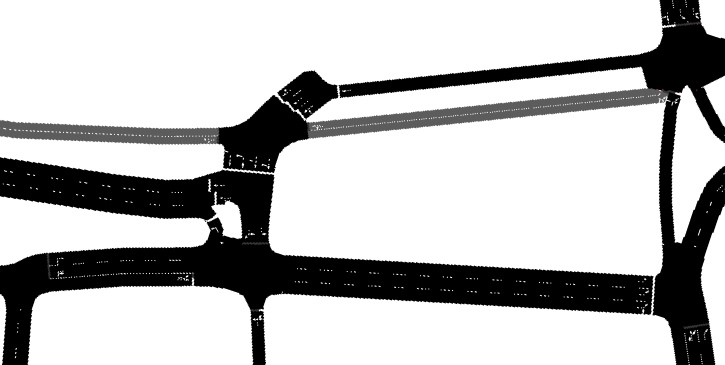
\includegraphics[width=0.70\textwidth]{images/cenario_estudo_sumo.png}

    \par\vspace{0.25cm}
    \begin{minipage}{0.70\textwidth}
        \footnotesize Fonte: Elaborado pelo autor.
    \end{minipage}
\end{figure}

\section{Ferramentas utilizadas}

Para o desenvolvimento deste trabalho, será utilizado o \gls{sumo}, do inglês \textit{Simulation of Urban MObility}, como ferramenta principal para a construção e execução das simulações microscópicas de tráfego. A ferramenta foi escolhida por ser \textit{open source}, permitir a representação individual dos veículos, possibilitar a configuração de parâmetros de condução e gerar arquivos de saída úteis para a análise dos resultados.

A rede viária inicial será baseada em dados do OpenStreetMap. Para sua preparação serão utilizados recursos do próprio \gls{sumo}, como o \textit{netconvert}, responsável pela conversão da rede para o formato do simulador, e o \textit{NetEdit}, utilizado para visualizar e editar vias, conexões, sentidos de circulação e permissões de conversão.

Também poderão ser utilizados \textit{scripts} em Python para auxiliar na automação das simulações, na alteração de parâmetros, na organização dos arquivos de saída e no tratamento dos dados obtidos. O ambiente previsto para o desenvolvimento desses \textit{scripts} será o Visual Studio Code. Para a análise dos resultados, poderão ser utilizadas bibliotecas Python voltadas ao tratamento de dados e geração de gráficos, como \textit{pandas} e \textit{matplotlib}.

\section{Construção do cenário de simulação}

A construção do cenário de simulação será realizada a partir do recorte urbano definido para o trabalho. Inicialmente, a rede viária será importada com base em dados do OpenStreetMap e convertida para o formato do \gls{sumo}. Essa rede será utilizada como ponto de partida para a modelagem do cenário.

Após a importação, a rede será analisada no \gls{sumo} e no \textit{NetEdit}. Essa etapa será necessária para verificar se a estrutura obtida está adequada às necessidades do cenário de simulação. Serão observados principalmente os sentidos das vias, as conexões entre os trechos, as permissões de conversão, a quantidade de faixas e os pontos de entrada e saída de veículos.

Caso sejam identificadas inconsistências, serão realizados ajustes manuais na rede. Esses ajustes serão importantes especialmente no entorno da Praça Nereu Ramos, pois a região possui diferentes possibilidades de deslocamento, mudanças de direção e aproximações entre fluxos. O objetivo será obter uma representação simplificada, mas funcional, da circulação no trecho analisado.

Também poderão ser feitas simplificações no cenário, removendo ou desconsiderando elementos que não contribuam diretamente para os objetivos do trabalho. Essa escolha busca manter o escopo viável, concentrando a análise nos trechos que influenciam a circulação principal da área estudada.

Depois da construção da rede, serão feitos testes preliminares no \gls{sumo} para verificar a coerência operacional do cenário. Nessa etapa, serão observados aspectos como continuidade das rotas, ausência de bloqueios indevidos, funcionamento das conexões entre vias, comportamento dos veículos nos pontos de entrada e saída e formação de filas decorrente da própria configuração simulada. Caso sejam identificados problemas, a rede será ajustada novamente até que esteja adequada para a configuração dos fluxos, perfis de motoristas e cenários de simulação.

\section{Definição dos perfis de motoristas}

Para analisar o impacto do comportamento dos condutores no tráfego urbano, serão definidos perfis de motoristas a serem utilizados nas simulações. Esses perfis serão representados por meio de parâmetros computacionais do \gls{sumo} relacionados à forma de condução dos veículos.

Inicialmente, serão considerados três perfis principais: cauteloso, normal e agressivo. O perfil cauteloso representará uma configuração com tendências mais conservadoras de condução, como maior distância de seguimento e menor aceitação de lacunas. O perfil normal será utilizado como referência intermediária, sem características extremas de condução. Já o perfil agressivo representará uma configuração com tendências opostas, como menor distância de seguimento, maior aceleração e maior aceitação de lacunas.

A definição desses perfis não tem como objetivo classificar todos os motoristas reais de forma definitiva. Trata-se de uma simplificação necessária para permitir a comparação entre cenários simulados. Dessa forma, os perfis serão utilizados como abstrações computacionais, permitindo observar como diferentes parâmetros de condução podem influenciar o desempenho do tráfego.

Entre os parâmetros que poderão ser utilizados para diferenciar os perfis estão aceleração, desaceleração, distância mínima de seguimento, velocidade desejada, tempo de reação ou seguimento e aceitação de lacunas. O Quadro~\ref{qua:perfis-motoristas} apresenta a tendência esperada desses parâmetros para cada perfil. Os valores concretos desses parâmetros não serão definidos de forma arbitrária. Na etapa de desenvolvimento do TCC, eles serão estabelecidos a partir da literatura relacionada à heterogeneidade de motoristas, dos parâmetros configuráveis disponíveis no \gls{sumo}, da documentação da ferramenta e de testes preliminares no cenário construído. A literatura será utilizada para orientar as tendências esperadas de cada perfil, como diferenças na distância de seguimento, na aceleração, na desaceleração e no tempo de reação dos motoristas \cite{ossen_2011,zhai_2021,mecheva_2022,makridis_2023}. Esses testes não terão como objetivo realizar uma calibração completa com dados reais de tráfego, mas verificar se os valores adotados produzem comportamentos coerentes para fins comparativos, sem gerar situações artificiais, como bloqueios indevidos, acelerações incompatíveis ou instabilidade na circulação. Os valores finais utilizados em cada perfil serão documentados no TCC, permitindo a reprodução dos cenários simulados.


\begin{quadro}[htbp]
\centering
\caption{Tendências esperadas dos parâmetros por perfil de motorista}
\label{qua:perfis-motoristas}
\small
\renewcommand{\arraystretch}{1.25}

\begin{tabular}{|p{5.4cm} | p{3.0cm} | p{2.8cm} | p{2.8cm}|}
\hline
\textbf{Parâmetro} & \textbf{Cauteloso} & \textbf{Normal} & \textbf{Agressivo} \\
\hline
Aceleração & Menor & Intermediária & Maior \\
\hline
Desaceleração & Mais conservadora & Intermediária & Mais intensa \\
\hline
Distância mínima de seguimento & Maior & Intermediária & Menor \\
\hline
Velocidade desejada & Menor & Intermediária & Maior \\
\hline
Tempo de reação ou seguimento & Maior & Intermediário & Menor \\
\hline
Aceitação de lacunas & Menor & Intermediária & Maior \\
\hline
\end{tabular}

\par\vspace{0.25cm}
\begin{minipage}{\textwidth}
\footnotesize Fonte: Elaborado pelo autor.
\end{minipage}

\end{quadro}

\section{Definição dos cenários de simulação}

Os cenários de simulação serão definidos a partir da combinação entre a rede viária construída, os níveis de fluxo de veículos e as composições dos perfis de motoristas configurados. A intenção é realizar comparações controladas, permitindo variar separadamente a intensidade do fluxo e a participação dos diferentes perfis de condução.

Inicialmente, serão considerados três níveis de fluxo: baixo, médio e alto. Esses níveis não terão como objetivo reproduzir exatamente a quantidade real de veículos da região estudada, mas representar diferentes condições de carregamento da rede. Os valores associados a cada nível serão definidos durante os testes preliminares, considerando o comportamento do cenário no \gls{sumo}.

Também serão consideradas diferentes composições dos perfis cauteloso, normal e agressivo. Além de cenários de referência compostos apenas por motoristas com perfil normal, serão avaliadas composições mistas, incluindo situações com distribuição mais equilibrada entre os perfis e situações com maior participação de determinado perfil. Os percentuais finais serão definidos após testes preliminares, buscando produzir diferenças suficientes para comparação sem criar configurações excessivamente artificiais.

Os cenários serão organizados de forma que seja possível comparar diferentes composições mantendo o mesmo nível de fluxo e, de forma complementar, comparar diferentes níveis de fluxo mantendo a mesma composição de perfis. Essa organização busca permitir uma análise mais clara dos efeitos associados ao comportamento dos motoristas e das alterações decorrentes do carregamento da rede.

\begin{quadro}[H]
\centering
\caption{Estrutura inicial dos cenários de simulação}
\label{qua:cenarios-simulacao}
\small
\renewcommand{\arraystretch}{1.25}

\begin{tabular}{|p{4.7cm}| p{3cm}| p{7.2cm}|}
\hline
\textbf{Tipo de cenário} & \textbf{Fluxo previsto} & \textbf{Composição prevista} \\
\hline
Referência & Baixo, médio e alto & Motoristas com perfil normal. \\
\hline
Composição mista equilibrada & Baixo, médio e alto & Participação semelhante dos perfis cauteloso, normal e agressivo. \\
\hline
Predominância cautelosa & Baixo, médio e alto & Maior participação de motoristas com perfil cauteloso. \\
\hline
Predominância agressiva & Baixo, médio e alto & Maior participação de motoristas com perfil agressivo. \\
\hline
\end{tabular}

\par\vspace{0.25cm}
\begin{minipage}{\textwidth}
\footnotesize Fonte: Elaborado pelo autor.
\end{minipage}

\end{quadro}

O Quadro~\ref{qua:cenarios-simulacao} apresenta a estrutura inicial prevista para os experimentos. As proporções dos perfis e os valores correspondentes aos níveis de fluxo ainda serão definidos durante a etapa prática do trabalho. Os testes preliminares serão utilizados para verificar quais configurações produzem condições adequadas para a comparação entre os cenários.

A execução dessas combinações permitirá observar tanto os efeitos associados à composição dos perfis de motoristas quanto as possíveis mudanças desses efeitos em diferentes condições de carregamento da rede. As configurações finais utilizadas nos experimentos serão documentadas no TCC para permitir a reprodução das simulações.

\section{Métricas de avaliação}

A avaliação dos cenários simulados será realizada por meio de métricas relacionadas ao desempenho do tráfego. Essas métricas serão obtidas a partir dos arquivos de saída gerados pelo \gls{sumo} após a execução das simulações. A escolha das métricas busca permitir a comparação entre os diferentes cenários e níveis de fluxo definidos no trabalho.

Entre as principais métricas previstas estão o tempo médio de viagem, a velocidade média, o tempo parado, a formação de filas e a vazão de veículos. O tempo médio de viagem será utilizado para observar quanto tempo, em média, os veículos levam para percorrer o cenário. A velocidade média permitirá avaliar a fluidez do tráfego, enquanto o tempo parado indicará situações em que os veículos permanecem retidos ou com deslocamento interrompido.

A formação de filas será considerada para identificar pontos de maior retenção no cenário, principalmente em trechos de aproximação, conversão ou entrada no fluxo. Já a vazão de veículos será utilizada para observar a quantidade de veículos que consegue atravessar ou concluir o percurso no período simulado. Essas métricas, analisadas em conjunto, permitirão avaliar as diferenças de desempenho do tráfego entre os cenários simulados.

Caso necessário, outras métricas disponibilizadas pelo \gls{sumo} poderão ser consideradas durante a etapa prática do trabalho, desde que estejam relacionadas aos objetivos da pesquisa. A definição final das métricas dependerá da viabilidade de extração dos dados e da relevância de cada informação para a comparação entre os cenários simulados.

\section{Procedimentos de análise dos resultados}

Após a execução das simulações, os dados gerados pelo \gls{sumo} serão organizados para permitir a comparação entre os cenários definidos. Essa etapa envolverá a leitura dos arquivos de saída, a seleção das métricas de interesse e a organização dos resultados em tabelas ou gráficos, de acordo com a necessidade da análise.

As comparações serão realizadas considerando tanto as diferentes composições de perfis de motoristas quanto os níveis de fluxo de veículos. Para analisar os efeitos associados aos perfis de condução, serão comparados cenários com diferentes composições mantendo o mesmo nível de fluxo. De forma complementar, cenários com a mesma composição serão comparados em diferentes níveis de fluxo, permitindo observar como o carregamento da rede pode influenciar os resultados.

Os cenários de referência, compostos por motoristas com perfil normal, serão utilizados como base para parte das comparações. A análise buscará identificar diferenças no tempo médio de viagem, na velocidade média, no tempo parado, na formação de filas e na vazão, considerando também se os efeitos das diferentes composições se tornam mais perceptíveis conforme aumenta a intensidade do fluxo.

Para reduzir a influência de variações ocasionais, serão realizadas múltiplas execuções de cada configuração utilizando diferentes sementes pseudoaleatórias definidas e registradas. Dessa forma, será possível considerar a variabilidade introduzida pelos elementos aleatórios da simulação e, ao mesmo tempo, manter um registro que permita reproduzir posteriormente as execuções realizadas. A quantidade de repetições será estabelecida após os testes preliminares, considerando a variabilidade e a estabilidade observadas nos resultados.

Os resultados das diferentes execuções poderão ser consolidados por meio de valores médios e outras formas de organização que se mostrarem adequadas durante a análise. A necessidade de procedimentos estatísticos adicionais será avaliada posteriormente, de acordo com as características e a variabilidade dos dados obtidos.

Por fim, os resultados serão discutidos com base nos objetivos definidos no trabalho. A análise buscará identificar como diferentes composições de perfis de motoristas influenciam o desempenho do tráfego urbano no cenário simulado e como esses efeitos se relacionam com os diferentes níveis de carregamento da rede.

\section{Limitações do estudo}

Este trabalho não tem como objetivo reproduzir com precisão absoluta o trânsito real da região estudada. A proposta é construir um cenário urbano simplificado, baseado em um recorte real, que permita comparar de forma controlada os efeitos de diferentes composições de perfis de motoristas no desempenho do tráfego.

Alguns fatores presentes no trânsito real poderão ser desconsiderados ou simplificados, como comportamento de pedestres, transporte coletivo, estacionamento, condições climáticas, acidentes, obras e variações reais de demanda ao longo do dia. Essas simplificações são necessárias para manter o escopo do trabalho compatível com os objetivos da pesquisa e com o tempo disponível para seu desenvolvimento.

\begin{figure}[htbp]
    \centering
    \captionstyle[\centering]{\centering}
    \caption{Etapas previstas para o desenvolvimento da pesquisa}
    \label{fig:fluxograma-metodologia}

    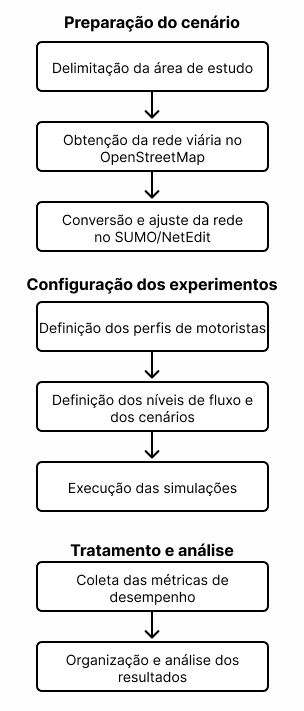
\includegraphics[width=0.32\textwidth]{images/fluxograma_metodologia.png}

    \par\vspace{0.15cm}
    \begin{minipage}{0.32\textwidth}
        \footnotesize Fonte: Elaborado pelo autor.
    \end{minipage}
\end{figure}

Dessa forma, os resultados obtidos deverão ser interpretados como uma análise comparativa entre cenários simulados, e não como uma previsão exata do funcionamento do trânsito da região. O foco estará na observação dos efeitos produzidos pelas diferentes composições de perfis de motoristas e pelos níveis de fluxo definidos para a simulação. A Figura~\ref{fig:fluxograma-metodologia} apresenta, de forma resumida, as etapas previstas para a execução da pesquisa.
% \chapter{CRONOGRAMA}

O cronograma a seguir apresenta uma previsão das principais etapas para o desenvolvimento do trabalho ao longo do período de execução do TCC. As atividades foram organizadas de forma a contemplar a revisão bibliográfica complementar, a construção do cenário de simulação, a realização dos experimentos, a análise dos resultados e a escrita final do trabalho.

\begin{quadro}[htbp]
\centering
\caption{Cronograma previsto para o desenvolvimento do TCC}
\label{qua:cronograma}
\small
\renewcommand{\arraystretch}{1.2}

\begin{tabular}{|p{9cm} | c | c | c | c | c | c|}
\hline
\textbf{Etapa} & \textbf{Jul} & \textbf{Ago} & \textbf{Set} & \textbf{Out} & \textbf{Nov} & \textbf{Dez} \\
\hline
Revisão bibliográfica complementar & X & X &  &  &  &  \\
\hline
Construção e ajuste da rede viária no \gls{sumo} & X & X &  &  &  &  \\
\hline
Definição dos perfis de motoristas &  & X & X &  &  &  \\
\hline
Definição dos fluxos e cenários de simulação &  & X & X &  &  &  \\
\hline
Execução das simulações &  &  & X & X &  &  \\
\hline
Coleta e organização dos dados &  &  &  & X & X &  \\
\hline
Análise dos resultados &  &  &  & X & X &  \\
\hline
Escrita e revisão do TCC &  & X & X & X & X & X \\
\hline
Preparação da apresentação e defesa &  &  &  &  &  & X \\
\hline
\end{tabular}

\par\vspace{0.25cm}
\begin{minipage}{\textwidth}
\footnotesize Fonte: Elaborado pelo autor.
\end{minipage}

\end{quadro}

A etapa de revisão bibliográfica complementar será voltada principalmente à busca de referências relacionadas à parametrização dos perfis de motoristas, às métricas de análise e ao uso do \gls{sumo} em estudos semelhantes. Embora a fundamentação teórica já tenha sido desenvolvida no PTC, essa revisão adicional será importante para apoiar a implementação prática da pesquisa.

Na etapa seguinte, será realizada a construção e o ajuste da rede viária no \gls{sumo}. Essa fase incluirá a obtenção da base inicial no OpenStreetMap, a conversão para o formato do simulador e os ajustes manuais necessários na rede, especialmente em sentidos de circulação, conexões e permissões de conversão.

Depois disso, serão definidos os perfis de motoristas, os níveis de fluxo e os cenários de simulação. Nessa fase, serão configurados os parâmetros de condução que representarão os perfis cauteloso, normal e agressivo, bem como os cenários de fluxo baixo, médio e alto.

Na sequência, serão executadas as simulações e realizada a coleta dos dados gerados pelo \gls{sumo}. Esses dados serão organizados para permitir a análise das métricas de desempenho, como tempo médio de viagem, velocidade média, tempo parado, formação de filas e vazão de veículos.

Por fim, será realizada a análise dos resultados, seguida da escrita e revisão final do TCC. A etapa final do cronograma será dedicada à preparação da apresentação e da defesa do trabalho.
% \chapter{RESULTADOS ESPERADOS}

Com o desenvolvimento deste trabalho, pretende-se construir um cenário de simulação microscópica baseado em um recorte urbano real da região central de Videira, permitindo analisar, de forma controlada, o impacto de diferentes perfis de motoristas sobre o desempenho do tráfego.

Como resultado inicial, busca-se obter uma rede viária funcional no \gls{sumo}, configurada de forma simplificada, mas suficiente para representar a dinâmica principal de circulação da área estudada. Também deverão ser definidos perfis de motoristas com características distintas de condução, possibilitando a criação de cenários comparativos com diferentes níveis de fluxo e diferentes composições de comportamento dos condutores.

Do ponto de vista analítico, o trabalho deverá permitir a comparação entre os perfis cauteloso, normal e agressivo a partir de métricas como tempo médio de viagem, velocidade média, tempo parado, formação de filas e vazão de veículos. A análise dos cenários simulados poderá indicar se determinados comportamentos produzem efeitos mais significativos sobre o tráfego, especialmente em situações de maior carregamento da rede.

Além disso, os resultados poderão contribuir para compreender como a variação de parâmetros comportamentais influencia o desempenho de um sistema viário urbano simulado. Dessa forma, a contribuição do trabalho não está em validar o uso do \gls{sumo} como ferramenta, mas em aplicar a simulação computacional para investigar um problema específico relacionado ao comportamento dos motoristas em um cenário urbano delimitado.

Por fim, pretende-se que a pesquisa forneça uma base metodológica para a continuidade do estudo no TCC, incluindo a configuração dos perfis, a execução dos cenários, a coleta das métricas e a análise comparativa dos resultados. Essa base poderá ser ampliada futuramente com novos parâmetros, outros recortes urbanos, diferentes tipos de veículos ou condições adicionais de simulação.

%
\chapter{PREPARAÇÃO DO CENÁRIO EXPERIMENTAL}

\section{Delineamento do estudo}

Este trabalho caracteriza-se como uma pesquisa aplicada, de abordagem quantitativa e com caráter experimental. A natureza aplicada está relacionada ao uso de conceitos e ferramentas de simulação computacional para investigar um problema específico de tráfego urbano. O objetivo não foi desenvolver um novo simulador, mas utilizar uma ferramenta existente para analisar como diferentes comportamentos de motoristas podem influenciar o desempenho do tráfego em condições controladas.

A abordagem quantitativa decorre da comparação dos cenários por meio de métricas numéricas extraídas das simulações. O caráter experimental, por sua vez, está associado à alteração controlada de fatores definidos no estudo, principalmente o nível de demanda e a composição dos perfis de motoristas. Essa organização permite comparar diferentes configurações mantendo os demais elementos do experimento constantes, de forma compatível com a definição de pesquisa experimental apresentada por \citeonline{gil_2002}.

O desenvolvimento foi organizado em duas etapas principais. A primeira correspondeu à preparação do cenário experimental, incluindo a construção e adequação da rede viária, a definição da demanda e a realização de testes preliminares de funcionamento e plausibilidade. A segunda etapa, apresentada no capítulo seguinte, compreendeu a definição dos perfis de motoristas, a composição dos cenários e a execução sistemática dos experimentos.

A simulação não teve como objetivo reproduzir de forma exata o trânsito real de Videira. O recorte urbano real foi utilizado como referência para construir um cenário simplificado e funcional, adequado à comparação entre comportamentos de condução. Dessa forma, os ajustes realizados durante a preparação do cenário foram tratados como verificações funcionais e ajustes de plausibilidade, e não como uma calibração empírica do tráfego da região.

\section{Área de estudo}

O cenário foi baseado em um recorte da região central de Videira, em Santa Catarina, com foco no entorno da Praça Nereu Ramos e em vias adjacentes. A região apresenta diferentes aproximações, conversões, mudanças de faixa e encontros entre fluxos com prioridades distintas, características que favorecem a observação das interações entre os veículos.

Embora a circulação ocorra ao redor de uma área central, o trecho não foi tratado como uma rotatória formal. A rede foi representada de acordo com sua organização viária, incluindo sentidos de circulação, conexões e regras de prioridade necessárias para o funcionamento do cenário no simulador.

O recorte também incluiu segmentos de entrada e saída além do entorno imediato da praça. Essa decisão permitiu que os veículos fossem inseridos antes de alcançar a área central e deixassem a rede após atravessá-la, evitando que as viagens começassem ou terminassem diretamente nos principais pontos de interação.

A Figura~\ref{fig:cenario-estudo-tc} apresenta a área utilizada como referência para a construção do cenário.

\begin{figure}[H]
    \centering
    \captionstyle[\centering]{\centering}
    \caption{Representação da área de estudo no SUMO}
    \label{fig:cenario-estudo-tc}

    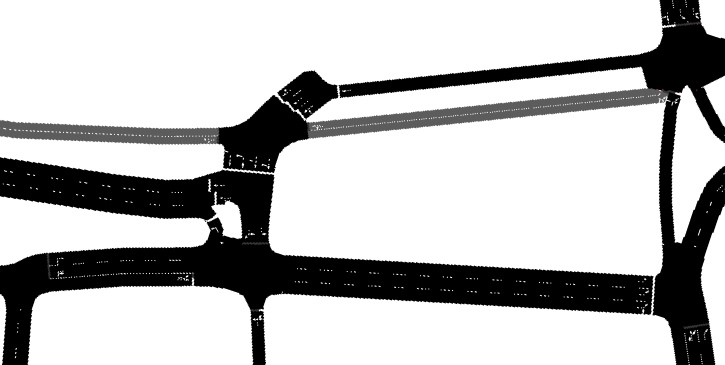
\includegraphics[width=0.70\textwidth]{images/cenario_estudo_sumo.png}

    \par\vspace{0.25cm}
    \begin{minipage}{0.70\textwidth}
        \footnotesize Fonte: Elaborado pelo autor.
    \end{minipage}
\end{figure}

\section{Construção e adequação da rede viária}

A rede inicial foi obtida a partir de dados do OpenStreetMap e convertida para o formato do \gls{sumo} com o \textit{netconvert}. A utilização de dados do OpenStreetMap como ponto de partida é compatível com o processo de construção de cenários descrito por \citeonline{clemente_2022}, que apresenta a preparação da rede, a definição do tráfego e o roteamento como etapas centrais de uma microssimulação no SUMO.

Após a conversão, a rede foi inspecionada e ajustada manualmente no \textit{NetEdit}. O objetivo dessa etapa foi obter uma representação funcional da circulação da região, e não preservar automaticamente todos os elementos importados. Foram removidos trechos externos sem função no experimento e corrigidos sentidos de circulação, conexões entre faixas, permissões de conversão, prioridades e geometrias que não estavam adequadas ao recorte utilizado.

Também foram revisadas as velocidades das vias. Na configuração utilizada nos experimentos, os limites ficaram concentrados em 40 km/h na região central e 50 km/h em trechos externos ou vias principais compatíveis com esse limite.

Um ajuste localizado foi realizado na região de acesso ao bairro Matriz, pela Rua Saul Brandalise. Na rede inicialmente importada, um veículo aguardando para realizar uma conversão à esquerda podia bloquear completamente o fluxo que seguia pela via. A observação do local mostrou a existência de um pequeno espaço utilizado para aguardar a conversão sem impedir necessariamente a passagem dos demais veículos. A geometria simulada foi então modificada para representar essa condição de forma simplificada.

A versão final da rede foi mantida em \texttt{config/nereu\_ramos.net.xml}. Versões anteriores foram preservadas no repositório do projeto para permitir rastrear os ajustes realizados durante o desenvolvimento.

\section{Verificação funcional do cenário}

Antes da definição dos experimentos, foram realizadas execuções preliminares para verificar se a rede permitia circulação contínua e se as conexões configuradas produziam trajetos válidos. Nessa etapa foram observados principalmente o funcionamento das entradas e saídas, o comportamento nos cruzamentos, as mudanças de faixa, as conversões e a formação de filas.

Os primeiros testes utilizaram viagens geradas com o \textit{randomTrips.py}. Essa estratégia foi útil para encontrar problemas de conectividade e comportamento da rede, mas também evidenciou uma limitação: uma distribuição totalmente aleatória atribuía tráfego excessivo a algumas vias secundárias e produzia uma utilização pouco plausível dos acessos da região. Por esse motivo, a geração de demanda foi posteriormente substituída por um procedimento controlado, descrito na seção seguinte.

A verificação também incluiu a observação de eventos que poderiam indicar problemas de configuração, como colisões, frenagens de emergência, bloqueios persistentes e \textit{teleports}. Os testes permitiram corrigir problemas localizados antes do congelamento da rede utilizada nos experimentos.

Durante a inspeção visual foi identificada ainda uma tendência de alguns veículos realizarem mudanças estratégicas de faixa com antecedência. Foram testadas alterações globais relacionadas ao comportamento estratégico de mudança de faixa, mas elas não produziram melhora suficiente para justificar sua adoção e, em alguns casos, introduziram instabilidade. Por esse motivo, a configuração-base foi mantida e essa característica foi considerada uma limitação conhecida da representação simulada.

\section{Definição e geração da demanda}

A demanda utilizada no experimento foi construída de forma controlada. O objetivo não foi reproduzir contagens reais de tráfego, pois não foi realizada uma coleta de fluxo veicular na região, mas evitar que a distribuição das viagens fosse completamente aleatória e pouco coerente com a importância relativa das vias do recorte.

As origens e os destinos foram definidos a partir dos acessos disponíveis na rede e receberam pesos relativos. As vias de maior importância no recorte receberam maior probabilidade de seleção, enquanto acessos secundários receberam pesos menores. Esses pesos representam apenas uma relação de importância entre os acessos e não correspondem a volumes reais medidos.

A Tabela~\ref{tab:pesos-demanda} apresenta os pesos utilizados na configuração final da demanda.

\begin{table}[H]
\centering
\caption{Pesos relativos utilizados na geração da demanda}
\label{tab:pesos-demanda}
\small
\renewcommand{\arraystretch}{1.20}
\begin{tabular}{|p{6.2cm}|c|c|}
\hline
\textbf{Via ou acesso} & \textbf{Peso como origem} & \textbf{Peso como destino} \\
\hline
Rua Saul Brandalise & 5 & 6 \\
\hline
Avenida Dom Pedro II & 5 & -- \\
\hline
Rua XV de Novembro -- acesso principal & 5 & 5 \\
\hline
Rua XV de Novembro -- acesso secundário & 3 & 4 \\
\hline
Rua Brasil & 3 & 3 \\
\hline
Rua Antônio Marafon & 2 & 1 \\
\hline
Rua Antônio Fávero & -- & 2 \\
\hline
Rua Osvaldo Cruz & 1 & 1 \\
\hline
Rua Santa Catarina & 1 & -- \\
\hline
Rua Padre Anchieta & -- & 1 \\
\hline
Rua Farroupilha & 1 & 1 \\
\hline
Rua Nicolau Cavon & 1 & 1 \\
\hline
Rua Sete de Setembro & -- & 1 \\
\hline
Rua Duque de Caxias & -- & 1 \\
\hline
\end{tabular}

\par\vspace{0.25cm}
\begin{minipage}{\textwidth}
\footnotesize Fonte: Elaborado pelo autor.
\end{minipage}
\end{table}

Além dos pesos individuais, alguns pares origem--destino receberam fatores de redução para diminuir a ocorrência de viagens que retornavam pelo mesmo corredor ou produziam deslocamentos pouco interessantes para o cenário. Em geral, retornos pelo mesmo corredor utilizaram fator 0,2. Os pares entre Rua Saul Brandalise e Rua Brasil, nos dois sentidos, utilizaram fator 0,6. Esses fatores reduzem a probabilidade de seleção dos pares, mas não os proíbem.

A geração foi implementada no script \texttt{scripts/gerar\_demanda\_v2.py}. Para cada execução, o script recebe a quantidade de veículos e uma semente pseudoaleatória. Os horários de partida são distribuídos uniformemente ao longo do intervalo de 0 a 600 segundos. Em seguida, a origem é sorteada de acordo com seus pesos e o destino é selecionado por uma distribuição ponderada condicionada à origem, considerando também os fatores aplicados aos pares penalizados.

Depois da geração das viagens, o \textit{duarouter} é utilizado para calcular rotas válidas na rede. O próprio processo verifica se a quantidade de rotas geradas corresponde à quantidade de veículos solicitada. Dessa forma, a aleatoriedade permanece na escolha das origens e destinos, mas ocorre dentro de uma estrutura de demanda controlada e reproduzível pela semente utilizada.

\section{Testes preliminares e ajustes de plausibilidade}

Durante os testes preliminares, um dos pontos que exigiu maior atenção foi o comportamento dos veículos em aproximações sem prioridade. Em determinadas situações, veículos permaneciam aguardando por períodos considerados excessivos mesmo quando existiam oportunidades visuais de entrada no fluxo prioritário. Esse comportamento produzia filas persistentes que dificultavam avaliar se a retenção era consequência da demanda ou da própria configuração do modelo de interseção.

Foram então avaliados parâmetros relacionados à aceitação de oportunidades em cruzamentos. O parâmetro global \texttt{time-to-impatience}, que controla a evolução da impaciência durante a espera, foi ajustado após testes comparativos. Na configuração final foi adotado o valor de 45 segundos. Também foi utilizado \texttt{jmTimegapMinor = 0.80}, relacionado ao intervalo temporal mínimo considerado na interação com veículos prioritários.

Esses valores não foram obtidos por calibração com dados reais da região. Eles foram mantidos como ajustes de plausibilidade após os testes mostrarem redução de esperas excessivamente conservadoras sem introduzir instabilidade generalizada na rede. A distinção é importante porque uma calibração empírica exigiria dados observados para comparar diretamente os comportamentos simulados com o trânsito real.

Outros parâmetros globais também foram mantidos constantes após essa etapa. O passo da simulação foi definido em 0,1 segundo, os \textit{teleports} foram desativados e a verificação de colisões em cruzamentos foi habilitada. Essas configurações permaneceram iguais entre os cenários para evitar que alterações no funcionamento básico do simulador interferissem na comparação entre os perfis de motoristas.

\section{Definição dos níveis de demanda}

A definição dos níveis de demanda foi realizada por meio de testes progressivos de carregamento da rede. O objetivo foi selecionar condições que representassem diferentes intensidades de circulação sem utilizar como cenário principal uma carga que produzisse congestionamento persistente ou impedisse a conclusão das viagens em determinadas realizações aleatórias.

Após os testes preliminares, foram definidos três níveis para o experimento: 300 veículos no nível baixo, 450 veículos no nível médio e 625 veículos no nível alto. Em todos os casos, os veículos são gerados durante a mesma janela de 600 segundos.

\begin{table}[H]
\centering
\caption{Níveis de demanda utilizados nos experimentos}
\label{tab:niveis-demanda}
\small
\renewcommand{\arraystretch}{1.20}
\begin{tabular}{|p{5cm}|c|c|}
\hline
\textbf{Nível} & \textbf{Veículos} & \textbf{Janela de geração} \\
\hline
Baixo & 300 & 0--600 s \\
\hline
Médio & 450 & 0--600 s \\
\hline
Alto & 625 & 0--600 s \\
\hline
\end{tabular}

\par\vspace{0.25cm}
\begin{minipage}{\textwidth}
\footnotesize Fonte: Elaborado pelo autor.
\end{minipage}
\end{table}

O nível de 300 veículos representa a condição de menor carregamento adotada no estudo. O nível de 450 veículos foi utilizado como condição intermediária. Para o nível alto, testes adicionais foram realizados com 625, 650, 675, 700 e 750 veículos. A carga de 625 veículos apresentou funcionamento estável nas repetições avaliadas durante o desenvolvimento, enquanto cargas superiores passaram a apresentar congestionamentos persistentes em algumas combinações de demanda e composição comportamental.

Por esse motivo, 625 veículos foi mantido como o nível alto do experimento principal. Essa escolha evita que o cenário de maior carregamento seja definido por uma condição em que parte das execuções deixa de representar apenas diferenças comportamentais e passa a ser dominada por um estado de congestionamento persistente da rede.

Com a rede, a demanda e os níveis de carregamento definidos, a configuração do cenário experimental foi congelada para a etapa seguinte. O próximo capítulo apresenta a parametrização dos perfis de motoristas, as composições utilizadas e o procedimento de execução das simulações.


% Os capítulos seguintes serão acrescentados conforme a escrita do TC:
% execução dos experimentos, resultados/discussão e conclusão.

% ----------------------------------------------------------
% ELEMENTOS PÓS-TEXTUAIS
% ----------------------------------------------------------
\postextual

% REFERÊNCIAS
\bibliography{referencias}

% APÊNDICES
% \begin{apendicesenv}

\chapter{Título do Apêndice A}

Arquivos confeccionados pelo autor do trabalho e que não se encaixam no texto.

 Ex: Deduções matemáticas, dimensionamentos extensos e algoritmos.

\end{apendicesenv}

% ANEXOS
% \begin{anexosenv}
\chapter{Título do Anexo A}
\label{anexoA}

Arquivos não confeccionados pelo autor do trabalho.


\end{anexosenv}

% ÍNDICE REMISSIVO
% \printindex

\end{document}
